\chapter{Optimal sr-paths}
\label{chapter:sr-optimal}

\section*{Introduction}

In this chapter we study several problems related to computing optimal sr-paths 
between two givens nodes. We start by defining weight functions for sr-paths and 
propose an algorithm for computing sr-paths of minimal weight with respect to such
a weight function and show how we can achieve low latency in a segment routed network. 
Next we study the reverse problem of finding a path of maximum
weight. Finally, we show how to compute sr-paths with maximum capacity. This is
useful to be able to route demands on a network without exceeding link capacities.

\section{Minimum weight sr-path}

The problem of computing minimum weight sr-paths appears 
in some form or another as a sub-problem in each of the three applications of segment routing
that we study in this thesis. It also has interesting applications in itself such as computing
sr-paths with minimum latency in the network or sr-paths with maximum bandwidth.

In order to be able to make sense of what we mean by a minimum weight sr-path, we need to define
weight functions for sr-paths which we call sr-metrics. These will essentially be generalizations of weight
function on graphs. To avoid confusion with minimum segment cost sr-paths, we will
always be careful to not interchange the words weight and cost. So whenever we mention the weight of a sr-path
we mean the value of some sr-metric when evaluated on that sr-path and whenever we mention its cost we are
thinking in terms of segments.

\begin{definition}
Let $G$ be a network. A \emph{sr-metric} is a function $w : \left( V(G) \times V(G) \right) \cup E(G) \rightarrow \mathbb{R} \cup \{ \infty \}$ such
that if there are no paths between $u$ and $v$ on $G$ then $w(u, v) = \infty$.
Given a sr-path $\sr{p} = \langle e_1, \ldots, e_n \rangle$ we define the weight $w(\sr{p})$ as
$$
w(\sr{p}) = \sum_{i = 2}^n w(x^2_{i - 1}, x^1_i) + \sum_{i : x_i \in E(G)} w(x_i).
$$
\end{definition}

The way to think about a sr-metric is that $w(u, v)$ for $u, v \in V(G)$ defines what we pay for traversing the shortest
paths between $u$ and $v$ and $w(e)$ for $e \in E(G)$ defines the weight of traversing edge $e$ with an adjacency segment.
The problem of finding minimum cost sr-paths with respect to some metric is defined as follows.

\begin{problem}{Minimum weight sr-path}
\label{problem:minweightsrpath}
\textbf{Input:} A network $G$, a sr-metric $w$, $k \in \mathbb{N}$ and two distinct nodes $s, t \in V(G)$.

\textbf{Output:} A sr-path $\sr{p} \in \mathcal{\sr{P}}_k(s, t)$ such that $w(\sr{p})$ is minimal.
\end{problem}

\subsection{General algorithm}

We propose in this section an algorithm for computing minimum weight sr-paths. The idea of this algorithm comes from
the Bellman-Ford shortest path algorithm \cite{Cormen:2009:IAT:1614191}. The Bellman-Ford algorithm is a dynamic programming (DP) algorithm
for computing shortest paths on graphs with both positive and negative edge weights from a given source $s$. At first sight, this might seem
totally different from what we are doing here. However if we look at the original dynamic programming formulation we see
that it is actually computing shortest paths of increasing lengths, in terms of edges. In a nutshell, they define DP
state spaces such that

\begin{align*}
\mathit{sol}(i, v) = \ & \textrm{the weight of the shortest path from} \\
            \ & \textrm{$s$ to $v$ using at most $i$ edges.}
\end{align*}

We are going to define a very similar state space in our solution. The main difference is that the
$i$ parameter will correspond the segment cost of the sr-path rather the a number of edges. We thus define the following DP state space

\begin{align*}
\mathit{sol}(i, v) = \ & \textrm{the minimum weight sr-path from} \\
            \ & \textrm{$s$ to $v$ with segment cost at most $i$.}
\end{align*}

The solution minimum weight sr-path problem is by definition $\mathit{sol}(k, t)$. For $i = 0$ the only possible sr-path of segment cost $0$ from $s$ to any node
is $\langle s \rangle$. Thus, we have that $\mathit{sol}(0, s) = 0$ and $\mathit{sol}(0, v) = \infty$ for $v \neq s$. 

The next step is to express $\mathit{sol}(i, *)$ in terms of $\mathit{sol}(j, s)$ with $j < i$.
The idea for doing this it to analyze the structure of a sr-path of cost $i$. There are three possibilities 
to reach a node $v$ with a sr-path of segment cost at most $i$.
These three possibilities are illustrated in Figure \ref{fig:dp}.
The first way is to simply not use
the extra segment and reach $v$ in the best way using a sr-path of segment cost at most
$i - 1$. The second possibility is to reach some node $u \in V$ using a sr-path of
segment cost at most $i - 1$ and then use one extra node segment to reach $v$ incurring an extra cost of $w(u, v)$. 
Finally, we can use a sr-path of cost at most $i - 2$ to any node $r$ and then append to it an adjacency
segment $(u, v)$ where $u$ is a in-neighbor of $v$. Note that nothing prevents $r$ from being equal to
$u$. In this case it simply means that we append the adjacency $(u, v)$ to a path that already ends at node
$u$. The cost increment of doing so is the cost of traversing the shortest path from $r$ to $u$ plus the cost
of the link $(u, v)$.

 \begin{figure}
 \begin{center}
 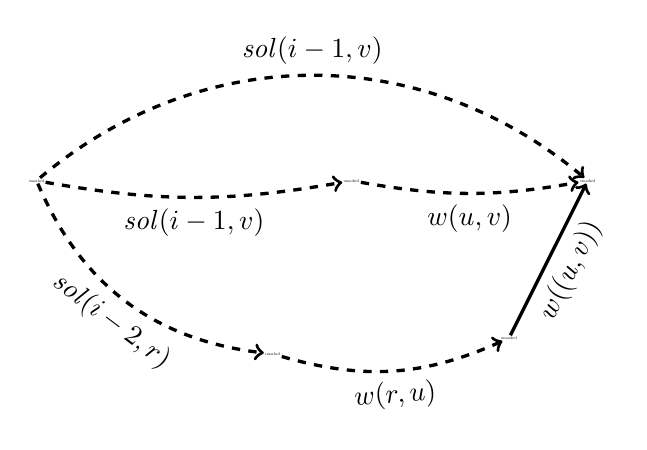
\begin{tikzpicture}
 \node[scale=0.15] (s) at (0, 0) {\router{s}{marked}};
 \node[scale=0.15] (x) at (5+2, 0) {\router{v}{marked}};
 \node[scale=0.15] (y) at (2+2, 0) {\router{u}{marked}};
 \node[scale=0.15] (z) at (4+2, -2) {\router{u}{marked}};
 \node[scale=0.15] (r) at (2+1, -2-0.2) {\router{r}{marked}};
 
 
 
 \draw (s) edge[very thick, below, bend right=10, dashed, ->] node {$\mathit{sol}(i - 1, v)$} (y);
 \draw (y) edge[very thick, bend right=10, dashed, ->, below] node {$w(u, v)$} (x);
 \draw (s) edge[very thick, bend left=40, dashed, ->, above] node {$\mathit{sol}(i - 1, v)$} (x);
 %\draw (s) edge[very thick, bend right=30, dashed, ->] (z);
 \draw (z) edge[very thick, ->, sloped, below] node {$w((u, v))$} (x);
 
 \draw (s) edge[very thick, bend right=30, dashed, ->, below, sloped] node {$\mathit{sol}(i - 2, r)$} (r);
 \draw (r) edge[very thick, bend right=20, dashed, ->, below, sloped] node {$w(r, u)$} (z);
 
 \end{tikzpicture}
 \end{center}
 \caption{Illustration of the $\mathit{sol}$ recurrence}
 \label{fig:dp}
 \end{figure}

The next theorem formalizes this intuition. 
 
\begin{theorem}
\label{thm:minwsrpath}
For $i \geq 1$ and $x \in V(G)$ it holds that

\small
\[\mathit{sol}(i, v) = \min \left\{
  \begin{matrix}
    \mathit{sol}(i - 1, v) &  \\[0.2cm]
    \mathit{sol}(i - 1, u)  +  w(u, v)  & s.t \text{ $y \in V$} \\[0.2cm]
    \mathit{sol}(i - 2, r)  +  w(r, u) + w((u, v)) & s.t \text{ $r \in V$} \\
\end{matrix}
  \right.
\]
\normalsize 
where the third value is only defined for $i \geq 2$ (set to $\infty$) otherwise.
\end{theorem}

\begin{proof}
Let $\sr{p} = \langle x_1, \ldots, x_n \rangle$ be a minimum weight sr-path from $s$ to $v$ of segment cost at most $i$. If 
$\cost(\sr{p}) < i$ then by definition $w(\sr{p}) = \mathit{sol}(i - 1, v)$. Suppose then
that $\cost(\sr{p}) = i$. We consider two cases.

\emph{Case 1: $x_n \in V(G)$}. In this case $\sr{q} = \langle x_1, \ldots, x_{n - 1} \rangle$ is a sr-path from $s$ to some node
$u = x^2_{n - 1}$ such that $w(\sr{q}) = i - 1$. It must be the case that $w(\sr{q}) = \mathit{sol}(i - 1, u)$ or otherwise 
we could replace it by a better sr-path and obtain a sr-path from $s$ to $v$ with lower weight. Therefore, by definition of $w$, we have
$$
\mathit{sol}(i, v) = w(\sr{p}) = w(\sr{q}) + w(u, v) = \mathit{sol}(i - 1, u) + w(u, v).
$$

\emph{Case 2: $x_n \in E(G)$}. This case is similar to the previous one. This time $\sr{q} = \langle x_1, \ldots, x_{n - 1} \rangle$ is a sr-path from $s$ to some node
$r = x^2_{n - 1}$ such that $w(\sr{q}) = i - 2$. Again, it must be the case that $w(\sr{q}) = \mathit{sol}(i - 2, r)$.
By definition of $w$, if we let $u = x^1_n$, it holds that
$$
\mathit{sol}(i, x) = w(\sr{p}) = w(\sr{q}) + w(x^2_{n - 1}, x^1_n) + w(x_n) = \mathit{sol}(i - 1, y) + w(r, u) + w((u, v)).
$$
\end{proof}

Since the values of $\mathit{sol}(i, *)$ depend only on $\mathit{sol}(i - 1, *)$, we can compute all these
values by iterating in increasing order of $i$. For each $i$, evaluating one state of the form
$(i, v)$ takes $O(|V(G)| + |V(G)| \cdot |\delta^-(v)|)$. Hence, given $i$, the cost of evaluating state $(i, v)$ 
all $v \in V(G)$ is $O(|V(G)|^2 + |V(G)| \cdot |E(G)|)$ making the total time complexity be $O(k \cdot |V(G)| \cdot |E(G)|)$.
A formalization of this algorithm is provided as Algorithm \ref{algo:min_weight_sr_path}.
Since this algorithm runs in polynomial time, we have the following result.

\begin{proposition}
Problem \ref{problem:minweightsrpath} can be solved in polynomial time. 
\end{proposition}

\begin{algorithm}[t]
\small
\caption{$\textsf{minWeightSrPath}\left( g, orig, dest, w, maxSeg \right)$}
\begin{algorithmic}[1]
\STATE $sol \gets \textsf{matrix}(maxSeg + 1, g.\textsf{V}(), \infty)$ \label{mwsrp-matrix}
\STATE $sol(0, orig) = 0$
\STATE $parent \gets \textsf{matrix}(maxSeg + 1, g.\textsf{V}(), \textbf{null})$
\FOR{$i = 1, \ldots, maxSeg$}
  \FOR{$cur \in g.\textsf{V}()$}
    \STATE $sol(i, cur) \gets sol(i - 1, cur)$
    \STATE $parent(i, cur) \gets parent(i - 1, cur)$
    \FOR{$prev \in g.\textsf{V}() \setminus \{ cur \}$} \label{mwsrp-for1}
      \IF{$sol(i - 1, prev) + w(prev, cur) < sol(i , cur)$} \label{mwsrp-if1}
        \cmtline{we reach $cur$ using node segment}
	\STATE $sol(i, cur) = sol(i - 1, prev) + w(prev, cur)$
	\STATE $parent(i, cur) \gets prev$
      \ENDIF
    \ENDFOR
    \cmtline{the third case is only defined for $i \geq 2$}
    \IF{$i \geq 2$}
      \FOR{$e = (orig, dest) \in g.\textsf{inEdges}(cur)$}
	\FOR{$prev \in g.\textsf{V}() \setminus \{ cur \}$} \label{mwsrp-for2}
	  \IF{$sol(i - 2, prev) + w(prev, orig) + w(e) < sol(i, cur)$} \label{mwsrp-if2}
	    \cmtline{we reach $cur$ using adjacency}
	    \STATE $sol(i, cur) = sol(i - 2, prev) + w(prev, orig) + w(e)$
	    \STATE $parent(i, cur) \gets e$
	  \ENDIF
	\ENDFOR
      \ENDFOR
    \ENDIF
  \ENDFOR
\ENDFOR
\STATE $opt \gets sol(maxSeg, dest)$
\STATE $k \gets maxSeg$
\WHILE{$k - 1 \geq 0 \textbf{ and } sol(k - 1, dest) = opt$}
  \STATE $k \gets k - 1$
\ENDWHILE
\RETURN $\textsf{SrPath}(parent, orig, dest, k, opt)$
\end{algorithmic}
\label{algo:min_weight_sr_path}
\end{algorithm}

% Bellman-Ford algorithm is known to admit an alternative implementation using a queue that makes it run much faster 
% in practice. This is know as the \emph{shortest path faster algorithm} (SPFA). Indeed, experiments show that the SPFA
% has a runtime comparable to Dijkstra's algorithm in practice. It has been proved that it worst case complexity is the same as
% the original Bellman-Ford algorithm but it is conjectured that its average run time is $O(|E|)$. No theoretical results have been proved to support this, only experimental
% ones. Motivated by this, we also provide an alternative implementaiton and evaluate it in practice to see
% how much time we can gain with with it.
% 
% The idea is that the for loops on lines \ref{mwsrp-for1} and \ref{mwsrp-for2} of Algorithm \ref{algo:min_weight_sr_path} makes some useless iterations.
% To see this, suppose that $sol(i, v) = sol(i - 1, v)$ for some $i$. Then, at iteration $i + 1$ it is useless to consider $prev = v$ on both these for loops.
% In order to avoid such iterations we will maintain a set of nodes $v$ for which $sol(i, v) < sol(i - 1, v)$ and only consider those nodes at iteration
% $i + 1$.

\subsection{Achieving minimum latency with SR}

In this section we explore the problem of computing and implementing minimum latency paths in a network.
In a typical network, routing is done using shortest path routing with respect to the IGP costs configured on the links.
These costs can be, to some extent, arbitrary and need not be related with the link latencies. This means that it can happen
that a suboptimal path is used for forwarding packets, with respect to the total time it takes the packets to travel from the 
origin to its destination. 

In Figure \ref{fig:minlat_example} we illustrate such an example in a real network. The IGP shortest path between routers
\node{a} and \node{c} is the one shown in the solid blue edges and has a total latency of $101.4$ milliseconds. On the other hand,
the path $(\node{a}, \node{d}, \node{e}, \node{c})$, represented by the green edges, only has a latency of $58.2$ milliseconds, that is,
it is 74\% faster. This path can be implemented with segment routing by adding, for instance, a detour towards router \node{d} before forwarding the traffic
to router \node{c}.

\begin{figure}
\begin{center}
\begin{tikzpicture}
\def\x{0}
\def\y{0}

\node[scale=0.15] (a) at (0 + \x,  0 + \y) {\router{a}{marked}};
\node[scale=0.15] (b) at (3 + \x,  0 + \y) {\router{b}{router}};
\node[scale=0.15] (c) at (6 + \x,  0 + \y) {\router{c}{marked}};
\node[scale=0.15] (d) at (0 + \x,  -2 + \y) {\router{d}{router}};
\node[scale=0.15] (e) at (6 + \x,  -2 + \y) {\router{e}{router}};

\draw[line width=2] (a) edge[above, sloped] node[black,font=\bfseries] {\footnotesize \texttt{975, 59.8}} (b);
\draw[line width=2] (b) edge[above, sloped] node[black,font=\bfseries] {\footnotesize \texttt{90, 41.6}} (c);
\draw[line width=2] (a) edge[above, sloped] node[black,font=\bfseries] {\footnotesize \texttt{5, 0.1}} (d);
\draw[line width=2] (d) edge[above, sloped] node[black,font=\bfseries] {\footnotesize \texttt{1001, 31.5}} (e);
\draw[line width=2] (e) edge[above, sloped] node[black,font=\bfseries] {\footnotesize \texttt{63, 26.6}} (c);

\node (a1) at (-1.3, -0.5) {};
\node (a2) at (-0.5, 1) {};

\node (b1) at (2.5, 1) {};
\node (b2) at (3.8, 0.9) {};

\node (c1) at (5.5, 1) {};
\node (c2) at (6.7, 0.7) {};
\node (c3) at (7.5, -0.5) {};

\node (e1) at (5.5, -1 - 2) {};
\node (e2) at (7.5, 0.5 - 2) {};

\node (d1) at (0.3, -3) {};


% \draw[line width=2] (a) edge[above, sloped] node[black,font=\bfseries] {\footnotesize \texttt{}} (a1);
% \draw[line width=2] (a) edge[above, sloped] node[black,font=\bfseries] {\footnotesize \texttt{}} (a2);
% \draw[line width=2] (d) edge[above, sloped] node[black,font=\bfseries] {\footnotesize \texttt{}} (d1);
% 
% \draw[line width=2] (b) edge[above, sloped] node[black,font=\bfseries] {\footnotesize \texttt{}} (b1);
% \draw[line width=2] (b) edge[above, sloped] node[black,font=\bfseries] {\footnotesize \texttt{}} (b2);
% 
% \draw[line width=2] (c) edge[above, sloped] node[black,font=\bfseries] {\footnotesize \texttt{}} (c1);
% \draw[line width=2] (c) edge[above, sloped] node[black,font=\bfseries] {\footnotesize \texttt{}} (c2);
% \draw[line width=2] (c) edge[above, sloped] node[black,font=\bfseries] {\footnotesize \texttt{}} (c3);
% 
% \draw[line width=2] (e) edge[above, sloped] node[black,font=\bfseries] {\footnotesize \texttt{}} (e1);
% \draw[line width=2] (e) edge[above, sloped] node[black,font=\bfseries] {\footnotesize \texttt{}} (e2);


\draw (a) edge[line width=2, cyan, above, ->, bend right = 20] (b);
\draw (b) edge[line width=2, cyan, above, ->, bend right = 20] (c);

\draw (a) edge[line width=2, seagreen, above, ->, bend right = 20] (d);
\draw (d) edge[line width=2, seagreen, above, ->, bend right = 10] (e);
\draw (e) edge[line width=2, seagreen, above, ->, bend right = 20] (c);

\draw (8, -1) edge[line width=2, above] node {$\igp, \lat$} (9, -1);

\end{tikzpicture}
\end{center}
\caption{A small subgraph of a real network where the IGP shortest path between two nodes paths is 74\% slower than the optimal path.}
\label{fig:minlat_example}
\end{figure}

Although this example shows that SR can sometimes make it possible to find much more efficient paths, our
experiments show that the average gain is actually much lower than the 74\% shown above and that this is
an outlier result. For every topology in our data set,
we computed for every pair of distinct nodes, the minimum latency path between them and computed the ratio
between this value and the latency of the IGP shortest path. Figure \ref{fig:minlat_box} shows a box plot of these ratios.
On the $x$-axis, we either have a single topology or a topology group, and on the $y$-axis we have the ratio between
the nominal latency (latency of the IGP shortest path) and minimum latency of any path connecting the same
origin and destination.
We aggregated the results for the Zoo topologies because this data set contains over
200 topologies making it impossible show all of them. The last box shows the aggregated results over all topologies.
We can observe that the average gain is only 8\%, much lower than our example.

However, it is still interesting to study the problem of finding minimum latency segment routing paths for two reasons.
First, even if the gain is not as significant as our above example on average, there is still something to be gained in terms 
of latency when using SR over IGP shortest path routing as the overhead of doing so is quite small since
SR does not require routers to maintain state.
Second, as we will see later, this problem appears in some form or another as a subproblem of other
problems that we have tackled in this thesis.

\begin{figure}
\begin{center}
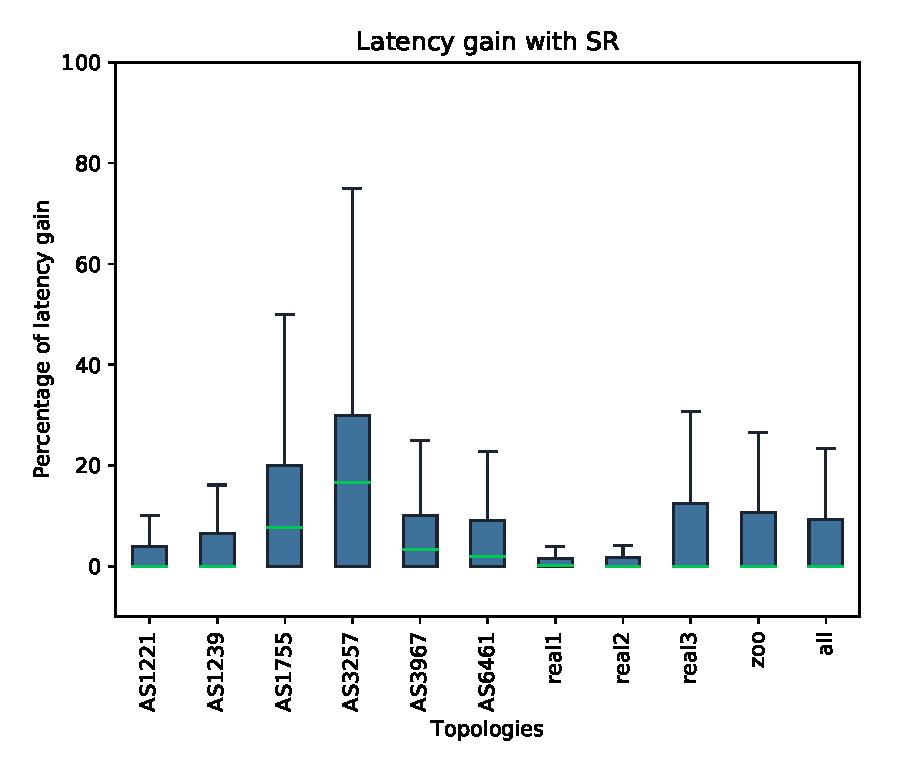
\includegraphics[scale=0.6]{./Network-lib/data/plot/minLat.eps}
\end{center}
\caption{Latecy gain in percentage.}
\label{fig:minlat_box}
\end{figure}

\subsubsection{Shortest path plus segmentation}

The first way to solve this problem with segment routing is to simply use a shortest path algorithm such as Dijkstra's algorithm
to compute the minimum latency path between the origin and the destination. Then, in order to implement that path with segment routing,
we can use the minimal segmentation algorithm proposed in Chapter \ref{chapter:sr} to segment that path.

The problem with doing this is that we have no control over the number of segments in the final path. If could be the case that the
minimum latency path actually requires a huge amount of segments to be implemented. Figure \ref{fig:minlat_seg} shows the distribution of
the number of segments required in the segmentation of the minimum latency paths over all pairs of nodes in the topologies from
our data set.

\begin{figure}
\begin{center}
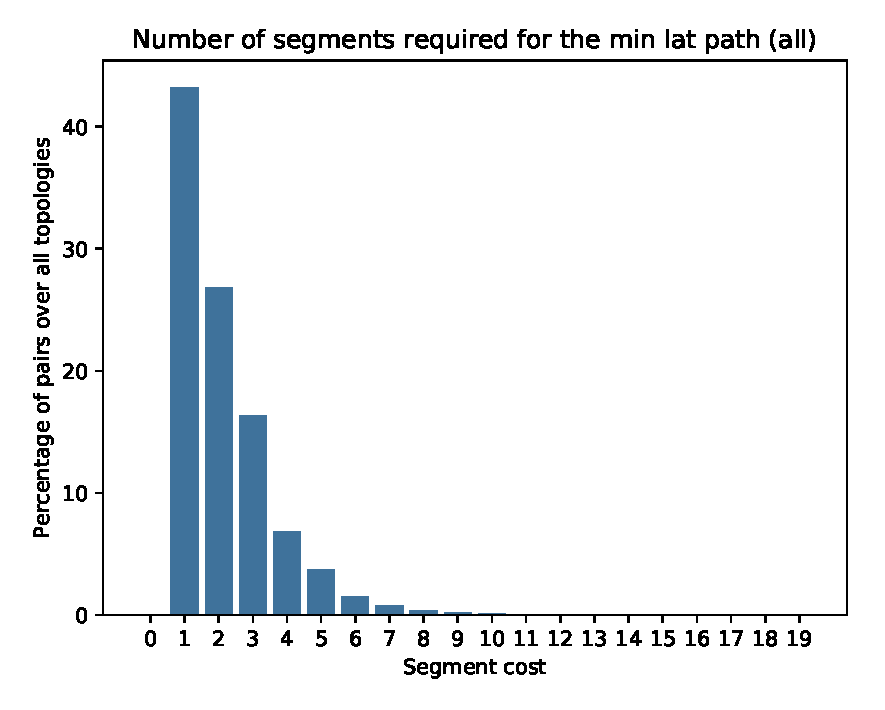
\includegraphics[scale=0.6]{./Network-lib/data/plot/minLat_seg.eps}
\end{center}
\caption{Number of segments required in the minimum latency paths over all topologies.}
\label{fig:minlat_seg}
\end{figure}

These results indicate that on average, there is some correlation between the IGP shortest paths and the
minimum latency paths. For $20$\% of the pairs over all topologies, the IGP shortest path matches the minimum latency
path. With about $5$ segments we can already route over $96$\% of the minimum latency paths. Thus we can say
that on average computing the minimum latency path and then segmenting it will yield a path that requires a small
segment stack and this is likely to be implementable on the network.

However, there are some topologies where this is far from true. Figure \ref{fig:minlat_seg_ovh} shows the same results
but for a single topology \topo{OVH-EUR}.

\begin{figure}
\begin{center}
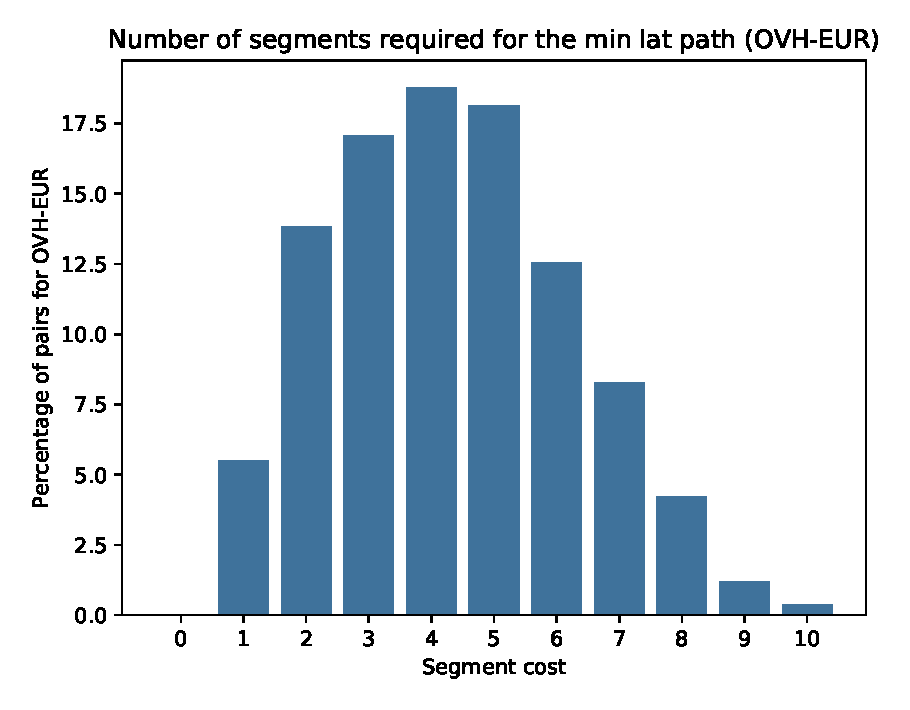
\includegraphics[scale=0.6]{./Network-lib/data/plot/minLat_seg_ovh.eps}
\end{center}
\caption{Number of segments required in the minimum latency paths for \topo{OVH-EUR}.}
\label{fig:minlat_seg_ovh}
\end{figure}

For this topology the situation is quite different as we need more than $5$ segments for about $26$\% of the pairs.
The reason why we observe this behavior in the \topo{OVH-EUR} topology is because it contains a lot of link
bundles having parallel links. This creates a lot of ECMP making it hard for segment routing to pass by
very specific paths.

This motivates the need for a minimum latency path finding algorithm that takes into account the number of 
segments from the start rather than simply computing a minimum latency path and hope that by chance it will
not requite a long segment stack.

%\todo{Talk about the case of equal cost latency. In this case maybe there is a path with less segments and equal latency.
%This is a bit technical, need to find a good way to talk about this.}

\subsubsection{Minimum latency SR-Path problem}

Another way of approaching this problem is to define a suitable sr-metric and use Algorithm \ref{algo:min_weight_sr_path} for computing a minimum 
latency sr-path. In this way
we will have full control over the number of segments in the output. The price to pay with this is that the latency of the obtained sr-path
will not be the global minimum but only the local minimum over all sr-paths in $\mathcal{\sr{P}}_k$.

To be able to define the problem more formally we need to define what is the latency of a sr-path.
This might seem obvious but in the presence of ECMP, a sr-path will correspond to a subnetwork of the original
network rather than a simple path. In reality, as we mentioned previously, the behavior of the network may vary making it impossible to
know which path amongst all paths defined by the sr-path will actually be used to forward traffic.

Let us illustrate this in a real example. Figure \ref{fig:spdag_ecmp} shows the shortest path subnetwork between routers \node{a} and \node{j} in a real network.
Both paths have the same IGP cost of $72$. The top path has latency $25.36ms$ and the bottom one has $19.1ms$.
Whenever we have a sr-path of the form $\langle \ldots, \node{a}, \node{j}, \ldots \rangle$, we do not know whether path $(\node{a}, \node{b}, \node{d}, \node{f}, \node{j})$ or $(\node{a}, \node{c}, \node{e}, \node{g}, \node{h}, \node{i}, \node{j})$
will be used to forward traffic between \node{a} and \node{j}.

\begin{figure}
\begin{center}
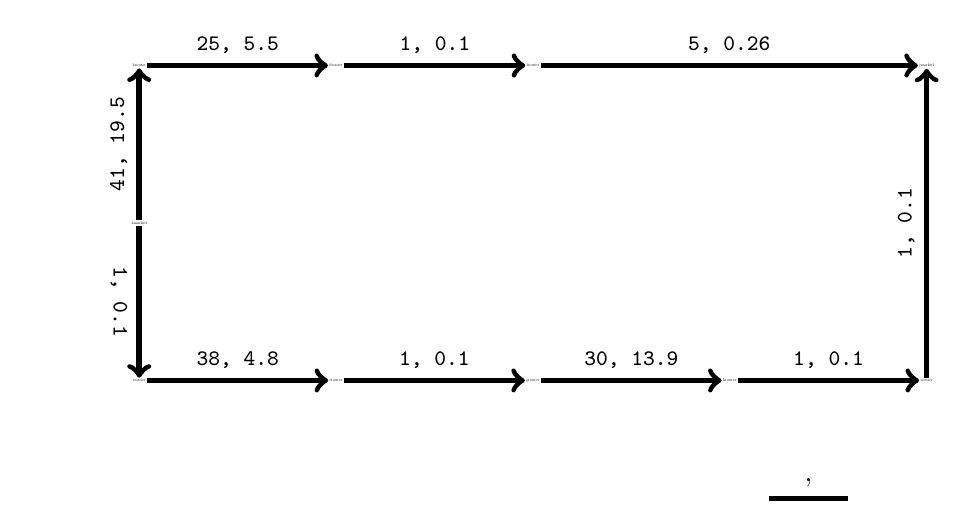
\begin{tikzpicture}
\def\x{0}
\def\y{0}

\node[scale=0.15] (a) at (0 + \x,  0 + \y) {\router{a}{marked}};
\node[scale=0.15] (b) at (0 + \x,  2 + \y) {\router{b}{router}};
\node[scale=0.15] (c) at (0 + \x,  -2 + \y) {\router{c}{router}};
\node[scale=0.15] (d) at (2.5 + \x,  2 + \y) {\router{d}{router}};
\node[scale=0.15] (e) at (2.5 + \x,  -2 + \y) {\router{e}{router}};
\node[scale=0.15] (f) at (5 + \x,  2 + \y) {\router{f}{router}};
\node[scale=0.15] (g) at (5 + \x,  -2 + \y) {\router{g}{router}};
\node[scale=0.15] (h) at (7.5 + \x,  -2 + \y) {\router{h}{router}};
\node[scale=0.15] (i) at (10 + \x,  -2 + \y) {\router{i}{router}};
\node[scale=0.15] (j) at (10 + \x,  2 + \y) {\router{j}{marked}};


\draw[line width=2] (a) edge[above, sloped, ->] node[black,font=\bfseries] {\footnotesize \texttt{41, 19.5}} (b);
\draw[line width=2] (b) edge[above, sloped, ->] node[black,font=\bfseries] {\footnotesize \texttt{25, 5.5}} (d);
\draw[line width=2] (d) edge[above, sloped, ->] node[black,font=\bfseries] {\footnotesize \texttt{1, 0.1}} (f);
\draw[line width=2] (f) edge[above, sloped, ->] node[black,font=\bfseries] {\footnotesize \texttt{5, 0.26}} (j);

\draw[line width=2] (a) edge[below, sloped, ->] node[black,font=\bfseries] {\footnotesize \texttt{1, 0.1}} (c);
\draw[line width=2] (c) edge[above, sloped, ->] node[black,font=\bfseries] {\footnotesize \texttt{38, 4.8}} (e);
\draw[line width=2] (e) edge[above, sloped, ->] node[black,font=\bfseries] {\footnotesize \texttt{1, 0.1}} (g);
\draw[line width=2] (g) edge[above, sloped, ->] node[black,font=\bfseries] {\footnotesize \texttt{30, 13.9}} (h);
\draw[line width=2] (h) edge[above, sloped, ->] node[black,font=\bfseries] {\footnotesize \texttt{1, 0.1}} (i);
\draw[line width=2] (i) edge[above, sloped, ->] node[black,font=\bfseries] {\footnotesize \texttt{1, 0.1}} (j);

\node (a1) at (-1.3, -0.5) {};
\node (a2) at (-0.5, 1) {};

\node (b1) at (2.5, 1) {};
\node (b2) at (3.8, 0.9) {};

\node (c1) at (5.5, 1) {};
\node (c2) at (6.7, 0.7) {};
\node (c3) at (7.5, -0.5) {};

\node (e1) at (5.5, -1 - 2) {};
\node (e2) at (7.5, 0.5 - 2) {};

\node (d1) at (0.3, -3) {};


\draw (8, -3.5) edge[line width=2, above] node {$\igp, \lat$} (9, -3.5);


% \draw[line width=2] (a) edge[above, sloped] node[black,font=\bfseries] {\footnotesize \texttt{}} (a1);
% \draw[line width=2] (a) edge[above, sloped] node[black,font=\bfseries] {\footnotesize \texttt{}} (a2);
% \draw[line width=2] (d) edge[above, sloped] node[black,font=\bfseries] {\footnotesize \texttt{}} (d1);
% 
% \draw[line width=2] (b) edge[above, sloped] node[black,font=\bfseries] {\footnotesize \texttt{}} (b1);
% \draw[line width=2] (b) edge[above, sloped] node[black,font=\bfseries] {\footnotesize \texttt{}} (b2);
% 
% \draw[line width=2] (c) edge[above, sloped] node[black,font=\bfseries] {\footnotesize \texttt{}} (c1);
% \draw[line width=2] (c) edge[above, sloped] node[black,font=\bfseries] {\footnotesize \texttt{}} (c2);
% \draw[line width=2] (c) edge[above, sloped] node[black,font=\bfseries] {\footnotesize \texttt{}} (c3);
% 
% \draw[line width=2] (e) edge[above, sloped] node[black,font=\bfseries] {\footnotesize \texttt{}} (e1);
% \draw[line width=2] (e) edge[above, sloped] node[black,font=\bfseries] {\footnotesize \texttt{}} (e2);
% 
% 
% \draw (a) edge[line width=2, cyan, above, ->, bend right = 20] (b);
% \draw (b) edge[line width=2, cyan, above, ->, bend right = 20] (c);
% 
% \draw (a) edge[line width=2, seagreen, above, ->, bend right = 20, dotted] (d);
% \draw (d) edge[line width=2, seagreen, above, ->, bend right = 10, dotted] (e);
% \draw (e) edge[line width=2, seagreen, above, ->, bend right = 20, dotted] (c);


\end{tikzpicture}
\end{center}
\caption{The shortest path DAG between routers \node{a} and \node{j} in a real network.}
\label{fig:spdag_ecmp}
\end{figure}

If we want to be able to provide guarantees about the latency, we need to consider the worst case scenario where, whenever
there is more than one path, we assume the slowest one is used. This corresponds to defining the latency of a sr-path
$\langle s_1, s_2 \rangle$ as the \emph{longest path} (w.r.t latencies) of any paths between $s_1$ and $s_2$ on $\sp(s_1, s_2)$.
This motivates the following definition.

\begin{definition}
Let $s_1, s_2$ be two nodes of a network $G$ and $e$ an edge.
The \emph{maximum latency sr-metric} is defined as
$$
\latmax(s_1, s_2) = \textrm{maximum latency of a path from $s_1$ to $s_2$ in $\sp(s_1, s_2)$}
$$
and
$$
\latmax(e) = \lat(e).
$$
\end{definition}

With this metric, we have $\latmax(\node{a}, \node{j}) = 25.38$. Note that on single edges this metric is defined as to
match that edge's latency. It is important to notice that this metric can be computed efficiently. It is well known that the
longest path problem is \textsf{NP}-hard in general \cite{Cormen:2009:IAT:1614191}. However, in this case we are computing it on an
acyclic network (the shortest path subnetwork) which can be done in linear time with a simple dynamic programming algorithm \cite{Cormen:2009:IAT:1614191}.

Another metric that is of interest is to consider that the latency of a sr-path is the average latency over all shortest paths.
This corresponds in practice with a situation where the next hops are selected randomly in case of ECMP. It somehow
reflects the behavior of selecting the next hops with an unknown hash function when several possible next hops exist.

\begin{definition}
Let $s_1, s_2$ be two nodes of a network $G$ and $e$ an edge.
The \emph{average latency sr-metric} is defined as
$$
\latavg(s_1, s_2) = \textrm{average latency among all paths from $s_1$ to $s_2$ in $\sp(s_1, s_2)$} 
$$
and
$$
\latavg(e) = \lat(e).
$$
\end{definition}

This metric can also be computed efficiently. We can use dynamic programming to compute the number of paths and their total
cost in linear time. The only complication is that this number grows exponentially which can easily be overcome using 
arbitrary precision integers.

Figure \ref{fig:ecmp_pc} shows the distribution of the number of equal cost shortest path between all pairs of routers over
all topologies. We can see about $60$\% of the time there is a single shortest path between the pairs of nodes. 
The maximum number of paths found for any pair of nodes was $11150$. This value might seem huge but it is actually quite small
when we take into the fact the number of paths in a DAG can be as large as $2^{|V| - 2}$ where $|V|$ is the number of routers in
that topology. This means that when computing average measures, we can probably use normal integers rather than arbitrary precision integers.

\begin{figure}
\begin{center}
\includegraphics[scale=0.6]{./Network-lib/data/plot/ecmpPathCount.eps}
\end{center}
\caption{Evaluation of the average number of ECMP over all topologies.}
\label{fig:ecmp_pc}
\end{figure}

\section{Maximum weight sr-paths}

In this section, we briefly discuss the problem of finding maximum weight sr-paths. 

\begin{problem}{Maximum weight sr-path}
\label{problem:maxweightsrpath}
\textbf{Input:} A network $G$, a sr-metric $w$, an integer constant $k \geq 1$ and two distinct nodes $s, t \in V(G)$.

\textbf{Output:} A sr-path $\sr{p} \in \mathcal{\sr{P}}_k(s, t)$ such that $w(\sr{p})$ is maximal.
\end{problem}

This problem can be solved in the exact same way as the minimum weight sr-path problem (Problem \ref{problem:minweightsrpath})
by replacing the $\infty$ by $-\infty$ on line \ref{mwsrp-matrix} and replacing the $<$ by $>$ on lines \ref{mwsrp-if1} and
\ref{mwsrp-if2} of Algorithm \ref{algo:min_weight_sr_path}.

This result might seem unintuitive at first because, as mentioned at the end of Chapter \ref{chapter:sr}, the longest path problem on graphs is \NPhard. Hence,
one might think by setting $k$ arbitrarily high and by using an appropriate sr-metric the two problems could become the same. There
is however an important nuance. In this problem we are not preventing the sr-path from repeating segments while the longest path
problem required simple paths. It is not hard to see that if we drop the simple path constraint then the longest path problem becomes trivial:
if the input graph is acyclic then we compute the answer with dynamic programming otherwise the answer is $\infty$ since we can
traverse any cycle an arbitrary amount of times getting longer and longer paths.

The next question one might then ask about this problem is, can this problem be interesting for some sr-metric $w$? The answer
is yes as we will see in Chapter \ref{chapter:scmon}.

\section{Maximum capacity sr-paths}

When routing traffic over a network it can be the case that the network is highly loaded. This can cause some network links
to become congested such as for instance, shortest path links or the links in the minimum latency path. Motivated by this,
we study the problem of finding a sr-path between two nodes whose congestion in minimum. Having such an algorithm can be
an interesting building block for dynamically allocating incoming demands while doing a best effort to prevent congestion.
Of course, using such an algorithm locally for each incoming demand will lead to an overall sub-optimal solution. We will
study the problem of considering all demands at once on Chapter \ref{chapter:te}.

We start with a very simple definition of demand.

\begin{definition}
A \emph{demand} in a network $G$ is a triple $(s, t, \nu)$ where $s, t \in V(G)$ and $\nu \in \mathbb{N}^+$. Given a demand $d$
we write $\src(d) = s$, $\dst(d) = t$ and $\vol(d) = \nu$.
\end{definition}

Before formally defining the problem that we solve in this section, we need to understand how traffic on a sr-path affects 
link loads since sr-paths can actually correspond to
several paths on the original network in case of ECMP. In this section we assume that the network is using a traffic split 
mechanism. Recall that this means that in the presence of ECMP,
the routers evenly split the incoming traffic amongst those equal cost paths. Consider sending one unit of flow
from node \node{a} to node \node{d} on the graph shown in Figure \ref{fig:split-example}. There are two shortest
paths between these nodes: $((\node{a}, \node{c}), (\node{c}, \node{d}))$ and $((\node{a}, \node{b}), (\node{b}, \node{d}))$.
Therefore, there will be a 50-50 split of the load over these two paths.

\begin{figure}[H]
\begin{center}
\begin{tikzpicture}[scale=1.2]
%\node[draw, circle] (a) at (0, 0) {\tiny \texttt{a}};

\node[scale=0.15] (a) at (0, 0)     {\router{a}{marked}};
\node[scale=0.15] (b) at (1, -1)    {\router{b}{router}};
\node[scale=0.15] (c) at (1, 1)     {\router{c}{router}};
\node[scale=0.15] (d) at (3, -1)    {\router{d}{marked}};
\node[scale=0.15] (e) at (3.5, 1.5) {\router{e}{router}};
\node[scale=0.15] (f) at (3.5, 0)   {\router{f}{router}};
\node[scale=0.15] (g) at (5, 1)     {\router{g}{router}};
\node[scale=0.15] (h) at (5, -1)    {\router{h}{router}};
\node[scale=0.15] (i) at (6, 0)     {\router{i}{router}};
\node[scale=0.15] (j) at (7.5, 0.5) {\router{j}{router}};
\node[scale=0.15] (k) at (7.5, -1)  {\router{k}{router}};

\draw[line width=2] (a) edge[above, sloped] node[black,font=\bfseries] {\footnotesize \texttt{$50\%$}} (c);
\draw[line width=2] (c) edge[above, sloped] node[black,font=\bfseries] {\footnotesize \texttt{$50\%$}} (d);
\draw[line width=2] (a) edge[above, sloped] node[black,font=\bfseries] {\footnotesize \texttt{$50\%$}} (b);
\draw[line width=2] (b) edge[above, sloped] node[black,font=\bfseries] {\footnotesize \texttt{$50\%$}} (d);


\draw[line width=2] (c) edge[above, sloped] node[black,font=\bfseries] {\footnotesize \texttt{}} (e);
\draw[line width=2] (c) edge[above, sloped] node[black,font=\bfseries] {\footnotesize \texttt{}} (f);
\draw[line width=2] (c) edge[above, sloped] node[black,font=\bfseries] {\footnotesize \texttt{}} (d);
\draw[line width=2] (e) edge[above, sloped] node[black,font=\bfseries] {\footnotesize \texttt{}} (g);
\draw[line width=2] (f) edge[above, sloped] node[black,font=\bfseries] {\footnotesize \texttt{}} (g);
\draw[line width=2] (f) edge[above, sloped] node[black,font=\bfseries] {\footnotesize \texttt{}} (h);
\draw[line width=2] (d) edge[above, sloped] node[black,font=\bfseries] {\footnotesize \texttt{}} (h);
\draw[line width=2] (g) edge[above, sloped] node[black,font=\bfseries] {\footnotesize \texttt{}} (i);
\draw[line width=2] (h) edge[above, sloped] node[black,font=\bfseries] {\footnotesize \texttt{}} (i);
\draw[line width=2] (i) edge[above, sloped] node[black,font=\bfseries] {\footnotesize \texttt{}} (j);


\draw[line width=2] (a) edge[above, sloped] node[black,font=\bfseries] {\footnotesize \texttt{}} (b);
\draw[line width=2] (b) edge[above, sloped] node[black,font=\bfseries] {\footnotesize \texttt{}} (d);
\draw[line width=2] (h) edge[above, sloped] node[black,font=\bfseries] {\footnotesize \texttt{}} (k);
\draw[line width=2] (i) edge[above, sloped] node[black,font=\bfseries] {\footnotesize \texttt{}} (k);
\draw[line width=2] (j) edge[above, sloped] node[black,font=\bfseries] {\footnotesize \texttt{}} (k);


\draw[line width=2] (a) edge[above, sloped] node[black,font=\bfseries] {\tiny \texttt{}} (b);
\draw[line width=2] (b) edge[above, sloped] node[black,font=\bfseries] {\tiny \texttt{}} (d);
\draw[line width=2] (k) edge[above, sloped] node[black,font=\bfseries] {\tiny \texttt{}} (h);
\draw[line width=2] (k) edge[above, sloped] node[black,font=\bfseries] {\tiny \texttt{}} (i);
\draw[line width=2] (k) edge[above, sloped] node[black,font=\bfseries] {\tiny \texttt{}} (j);

\draw (a) edge[line width=2, darkgreen, above, ->, bend right = 10] (b);
\draw (a) edge[line width=2, darkgreen, above, ->, bend right = 10] (c);
\draw (c) edge[line width=2, darkgreen, above, ->, bend right = 10] (d);
\draw (b) edge[line width=2, darkgreen, above, ->, bend right = 10] (d);

\node[left = 0.1cm of a, draw, fill=green] {\small $x_1$};
\node[below = 0.1cm of d, draw, fill=green] {\small $x_2$};

\end{tikzpicture}
\end{center}
\caption{Traffic split example between ECMP.}
\label{fig:split-example}
\end{figure}

We model this by computing, for each source-destination pair $s, t \in V(G)$, and every edge $e \in E(G)$,
what is the fraction of the traffic passing by $e$ when using shortest path routing from $s$ to $t$. In the previous example,
this fraction is $0.5$ for edges $\edge{a}{b}, \edge{a}{c}, \edge{c}{d}$ and $\edge{b}{d}$ and $0$ on all other edges
with $s = \node{a}$ and $t = \node{d}$. First, need to define the load on the nodes assuming that $1$ unit of traffic
is sent from $s$ to $t$.

\begin{definition}
Let $G$ be a network and $s, t \in V(G)$.  We define for every $v \in V(G)$
\[ \load^{st}(v) =
  \begin{cases}
    1      & \quad \text{if } v = s \\
    \displaystyle \sum_{u \in \delta^-(\sp(s, t), v)} \frac{\load(u)}{|\delta^+(\sp(s, t), u)|}  & \quad \text{otherwise}
  \end{cases}
\]
\end{definition}

Note that for each $s, t \in V(G)$, $\sp(s, t)$ is an acyclic graph so $\load^{st}(v)$ is well defined (it is not defined in terms of itself). 
The value of $\load^{st}(v)$ corresponds to the amount of traffic that would pass by the router corresponding to node
$v$ when routing one unit of traffic from $s$ to $t$, assuming that in case of ECMP the traffic is split equally. 
For example, consider the network shown in Figure \ref{fig:load} and assume
that $s = \node{c}$ and $t = \node{i}$ (shown in green). Then $\sp(s, t) = \sp(\node{c}, \node{i})$ corresponds to the green edges and the value of 
$\load^{st}(v)$ is shown in the gray boxes next to each node $v \in V(G)$. We see that, for instance, $\load^{st}(\node{h}) = 1 \slash 2$.
This means that under equal split, half of the traffic load sent with shortest path routing from \node{c} to \node{i}
will pass by \node{h}. This corresponds to the definition since
\begin{align*}
\load^{\node{c}\node{i}}(\node{h}) & = \sum_{u \in \delta^-(\sp(\node{c}, \node{i}), \node{h})} \frac{\load(u)}{|\delta^+(\sp(\node{c}, \node{i}), u)|} \\
& = \frac{1}{2} \cdot \load^{\node{c}\node{i}}(\node{f})  + \frac{1}{1} \cdot \load^{\node{c}\node{i}}(\node{d}) \\
& = \frac{1}{2} \cdot \frac{1}{3} + \frac{1}{3} = \frac{1}{6} + \frac{1}{3} = \frac{1}{2} \\
\end{align*}

\begin{figure}[H]
\begin{center}
\begin{tikzpicture}[scale=1.2]
%\node[draw, circle] (a) at (0, 0) {\tiny \texttt{a}};

\node[scale=0.15] (a) at (0, 0)     {\router{a}{router}};
\node[scale=0.15] (b) at (1, -1)    {\router{b}{router}};
\node[scale=0.15] (c) at (1, 1)     {\router{c}{marked}};
\node[scale=0.15] (d) at (3, -1)    {\router{d}{router}};
\node[scale=0.15] (e) at (3.5, 1.5) {\router{e}{router}};
\node[scale=0.15] (f) at (3.5, 0)   {\router{f}{router}};
\node[scale=0.15] (g) at (5, 1)     {\router{g}{router}};
\node[scale=0.15] (h) at (5, -1)    {\router{h}{router}};
\node[scale=0.15] (i) at (6, 0)     {\router{i}{marked}};
\node[scale=0.15] (j) at (7.5, 0.5) {\router{j}{router}};
\node[scale=0.15] (k) at (7.5, -1)  {\router{k}{router}};

\node[above = 0.1cm of c, draw, fill=green] {\small $x_1$};
\node[above = 0.1cm of i, draw, fill=green] {\small $x_2$};


\draw[line width=2] (a) edge[above, sloped] node[black,font=\bfseries] {\footnotesize \texttt{}} (c);
\draw[line width=2] (c) edge[above, sloped] node[black,font=\bfseries] {\footnotesize \texttt{}} (e);
\draw[line width=2] (c) edge[above, sloped] node[black,font=\bfseries] {\footnotesize \texttt{}} (f);
\draw[line width=2] (c) edge[above, sloped] node[black,font=\bfseries] {\footnotesize \texttt{}} (d);
\draw[line width=2] (e) edge[above, sloped] node[black,font=\bfseries] {\footnotesize \texttt{}} (g);
\draw[line width=2] (f) edge[above, sloped] node[black,font=\bfseries] {\footnotesize \texttt{}} (g);
\draw[line width=2] (f) edge[above, sloped] node[black,font=\bfseries] {\footnotesize \texttt{}} (h);
\draw[line width=2] (d) edge[above, sloped] node[black,font=\bfseries] {\footnotesize \texttt{}} (h);
\draw[line width=2] (g) edge[above, sloped] node[black,font=\bfseries] {\footnotesize \texttt{}} (i);
\draw[line width=2] (h) edge[above, sloped] node[black,font=\bfseries] {\footnotesize \texttt{}} (i);
\draw[line width=2] (i) edge[above, sloped] node[black,font=\bfseries] {\footnotesize \texttt{}} (j);

\draw[line width=2] (a) edge[above, sloped] node[black,font=\bfseries] {\tiny \texttt{}} (b);
\draw[line width=2] (b) edge[above, sloped] node[black,font=\bfseries] {\tiny \texttt{}} (d);
\draw[line width=2] (k) edge[above, sloped] node[black,font=\bfseries] {\tiny \texttt{}} (h);
\draw[line width=2] (k) edge[above, sloped] node[black,font=\bfseries] {\tiny \texttt{}} (i);
\draw[line width=2] (k) edge[above, sloped] node[black,font=\bfseries] {\tiny \texttt{}} (j);

\draw (c) edge[line width=2, darkgreen, above, ->, bend right = 10] (e);
\draw (c) edge[line width=2, darkgreen, above, ->, bend right = 10] (f);
\draw (c) edge[line width=2, darkgreen, above, ->, bend right = 10] (d);
\draw (e) edge[line width=2, darkgreen, above, ->, bend right = 10] (g);
\draw (f) edge[line width=2, darkgreen, above, ->, bend right = 10] (g);
\draw (f) edge[line width=2, darkgreen, above, ->, bend right = 10] (h);
\draw (d) edge[line width=2, darkgreen, above, ->, bend right = 10] (h);
\draw (g) edge[line width=2, darkgreen, above, ->, bend right = 10] (i);
\draw (h) edge[line width=2, darkgreen, above, ->, bend right = 10] (i);

\node[draw, fill=lightgray] at (c.south east) {\footnotesize $1$};
\node[draw, fill=lightgray] at (e.south east) {\tiny $1\slash3$};
\node[draw, fill=lightgray] at (f.south east) {\tiny $1\slash3$};
\node[draw, fill=lightgray] at (d.south east) {\tiny $1\slash3$};
\node[draw, fill=lightgray] at (g.south east) {\tiny $1\slash2$};
\node[draw, fill=lightgray] at (h.south east) {\tiny $1\slash2$};
\node[draw, fill=lightgray] at (i.south east) {\footnotesize $1$};

\node[draw, fill=lightgray] at (a.south east) {\footnotesize $0$};
\node[draw, fill=lightgray] at (b.south east) {\footnotesize $0$};
\node[draw, fill=lightgray] at (j.south east) {\footnotesize $0$};
\node[draw, fill=lightgray] at (k.south east) {\footnotesize $0$};


\end{tikzpicture}
\end{center}
\caption{Node loads with respect to $s = \node{c}$ and $t = \node{i}$.}
\label{fig:load}
\end{figure}

Using the node loads we can now define the edge loads which, as described above, give us the fraction of traffic traversed by a link
in the network. These values are necessary to express the link capacity constraints on TE models with segment routing. This is what we 
study in the next chapter.

\begin{definition}
Let $G$ be a network and $s, t \in V(G)$. We define, for every $e = (u, v) \in E(G)$
$$
\r(s, t, e) = \frac{\load^{st}(u)}{|\delta^+(\sp(s, t), u)|}.
$$
In order to characterize the proportion of traffic traversed by a link with respect to a sr-path $\sr{p} = \langle x_1, \ldots, x_n \rangle$ we define
$$
\r(\sr{p}, e) = \sum_{i = 2}^n \r(x^2_{i - 1}, x^1_i, e) + \sum_{i : x_i = e} 1.
$$
\end{definition}

The first part of the expression of $\r(\sr{p}, e)$ evaluates the ratio on $e$ for the shortest path subgraphs
between consecutive segments, while the second part counts how many times $e$ is used as an adjacency segment on the sr-path $\sr{p}$.
This summation is valid because when an adjacency segment occurs, the full unit demand is routed through the edge without split. 
Note that $\r(\sr{p}, e)$ may be larger than $1$ since a same edge can be used several times in case of cycles
in $\forw(\sr{p})$. Figure \ref{fig:ratio} shows the edge ratios $\r(\langle \node{a}, \node{c}, \node{i}, \node{j} \rangle, e)$ for
every $e \in E(G)$. The green arrows correspond to the forwarding graph of $\langle \node{a}, \node{c}, \node{i}, \node{j} \rangle$. 

\begin{figure}[H]
\begin{center}
\begin{tikzpicture}[scale=1.2]
%\node[draw, circle] (a) at (0, 0) {\tiny \texttt{a}};

\node[scale=0.15] (a) at (0, 0)     {\router{a}{marked}};
\node[scale=0.15] (b) at (1, -1)    {\router{b}{router}};
\node[scale=0.15] (c) at (1, 1)     {\router{c}{marked}};
\node[scale=0.15] (d) at (3, -1)    {\router{d}{router}};
\node[scale=0.15] (e) at (3.5, 1.5) {\router{e}{router}};
\node[scale=0.15] (f) at (3.5, 0)   {\router{f}{router}};
\node[scale=0.15] (g) at (5, 1)     {\router{g}{router}};
\node[scale=0.15] (h) at (5, -1)    {\router{h}{router}};
\node[scale=0.15] (i) at (6, 0)     {\router{i}{marked}};
\node[scale=0.15] (j) at (7.5, 0.5) {\router{j}{marked}};
\node[scale=0.15] (k) at (7.5, -1)  {\router{k}{router}};

\draw[line width=2] (a) edge[above, sloped] node[black,font=\bfseries] {\footnotesize \texttt{$1$}} (c);
\draw[line width=2] (c) edge[above, sloped] node[black,font=\bfseries] {\footnotesize \texttt{$1\slash3$}} (e);
\draw[line width=2] (c) edge[above, sloped] node[black,font=\bfseries] {\footnotesize \texttt{$1\slash3$}} (f);
\draw[line width=2] (c) edge[above, sloped] node[black,font=\bfseries] {\footnotesize \texttt{$1\slash3$}} (d);
\draw[line width=2] (e) edge[above, sloped] node[black,font=\bfseries] {\footnotesize \texttt{$1\slash3$}} (g);
\draw[line width=2] (f) edge[above, sloped] node[black,font=\bfseries] {\footnotesize \texttt{$1\slash6$}} (g);
\draw[line width=2] (f) edge[above, sloped] node[black,font=\bfseries] {\footnotesize \texttt{$1\slash6$}} (h);
\draw[line width=2] (d) edge[above, sloped] node[black,font=\bfseries] {\footnotesize \texttt{$1\slash3$}} (h);
\draw[line width=2] (g) edge[above, sloped] node[black,font=\bfseries] {\footnotesize \texttt{$1\slash2$}} (i);
\draw[line width=2] (h) edge[above, sloped] node[black,font=\bfseries] {\footnotesize \texttt{$1\slash2$}} (i);
\draw[line width=2] (i) edge[above, sloped] node[black,font=\bfseries] {\footnotesize \texttt{$1$}} (j);


\draw[line width=2] (a) edge[above, sloped] node[black,font=\bfseries] {\footnotesize \texttt{$0$}} (b);
\draw[line width=2] (b) edge[above, sloped] node[black,font=\bfseries] {\footnotesize \texttt{$0$}} (d);
\draw[line width=2] (h) edge[above, sloped] node[black,font=\bfseries] {\footnotesize \texttt{$0$}} (k);
\draw[line width=2] (i) edge[above, sloped] node[black,font=\bfseries] {\footnotesize \texttt{$0$}} (k);
\draw[line width=2] (j) edge[above, sloped] node[black,font=\bfseries] {\footnotesize \texttt{$0$}} (k);

\node[left = 0.1cm of a, draw, fill=green] {\small $x_1$};
\node[above = 0.1cm of c, draw, fill=green] {\small $x_2$};
\node[above = 0.3cm of i, draw, fill=green, anchor=west] {\small $x_3$};
\node[above = 0.1cm of j, draw, fill=green] {\small $x_4$};


\draw[line width=2] (a) edge[above, sloped] node[black,font=\bfseries] {\tiny \texttt{}} (b);
\draw[line width=2] (b) edge[above, sloped] node[black,font=\bfseries] {\tiny \texttt{}} (d);
\draw[line width=2] (k) edge[above, sloped] node[black,font=\bfseries] {\tiny \texttt{}} (h);
\draw[line width=2] (k) edge[above, sloped] node[black,font=\bfseries] {\tiny \texttt{}} (i);
\draw[line width=2] (k) edge[above, sloped] node[black,font=\bfseries] {\tiny \texttt{}} (j);

\draw (a) edge[line width=2, darkgreen, above, ->, bend right = 10] (c);
\draw (c) edge[line width=2, darkgreen, above, ->, bend right = 10] (e);
\draw (c) edge[line width=2, darkgreen, above, ->, bend right = 5] (f);
\draw (c) edge[line width=2, darkgreen, above, ->, bend right = 10] (d);
\draw (e) edge[line width=2, darkgreen, above, ->, bend right = 10] (g);
\draw (f) edge[line width=2, darkgreen, above, ->, bend right = 10] (g);
\draw (f) edge[line width=2, darkgreen, above, ->, bend right = 10] (h);
\draw (d) edge[line width=2, darkgreen, above, ->, bend right = 10] (h);
\draw (g) edge[line width=2, darkgreen, above, ->, bend right = 10] (i);
\draw (h) edge[line width=2, darkgreen, above, ->, bend right = 10] (i);
\draw (i) edge[line width=2, darkgreen, above, ->, bend right = 10] (j);


\end{tikzpicture}
\end{center}
\caption{Split ratio for sr-path $\langle \node{a}, \node{c}, \node{i}, \node{j} \rangle$.}
\label{fig:ratio}
\end{figure}

\begin{definition}
Let $G$ be a network and $\sr{p}$ a sr-path on $G$. We say that an edge $e \in E(\sr{p})$ is \emph{critical}
if the fraction $\frac{\bnd(e)}{\tau(\sr{p}, e)}$ has minimum value amongst all edges $e \in E(\sr{p})$.
We define the capacity of $\sr{p}$ as $\bnd(\sr{p}) = \min_{e \in E(\sr{p})} \frac{\bnd(e)}{\tau(\sr{p}, e)}$.
\end{definition}

To understand this definition, imagine that we route a demand $d$ over a sr-path $\sr{p}$.
The bandwidth that this will consume of each edge $e$ is given by $\tau(\sr{p}, e) \cdot \vol(d)$.
Hence, we will exceed the capacity of edge $e$ if and only if 
$$
\tau(\sr{p}, e) \cdot \vol(d) > \bnd(e) \Leftrightarrow \vol(d) > \frac{\bnd(e)}{\tau(\sr{p}, e)} .
$$
Hence $\bnd(\sr{p})$ describes the maximum volume that can be routed over $\sr{p}$ without exceeding the
capacity of any edge in $E(\sr{p})$.

% The capacity of a sr-path evaluates the maximum about of volume that can be routed over is whilst avoiding
% to exceed the capacity of any edge. It is not hard to see that if $\sr{p} = \langle x_1, \ldots x_n \rangle$
% then
% $$
% \bnd(\sr{p}) = \min_{e \in E(\sr{p})} \crit(e) = 
% $$

\begin{lemma}
\label{lemma:srcap}
Let $G$ be a network and $\sr{p} = \langle x_1, \ldots, x_n \rangle$ a sr-path on $G$. The following holds:
\begin{enumerate}[i)]
 \item If $x_n \in V(G)$ then $\bnd(\sr{p}) = \min \left( \bnd \langle x_1, \ldots, x_{n - 1} \rangle, \bnd \langle x^2_{n - 1}, x_n \rangle \right)$
 \item If $x_n \in E(G)$ then $\bnd(\sr{p}) = \min \left( \bnd \langle x_1, \ldots, x_{n - 1} \rangle, \bnd \langle x^2_{n - 1}, x^1_n \rangle, \bnd(x_n) \right)$
\end{enumerate}
\end{lemma}

\begin{proof}
Immediate from the definition of $\bnd(\sr{p})$ since in the first case we have 
$$
E(\sr{p}) = E(\langle x_1, \ldots, x_{n - 1} \rangle) \cup E(\langle x^2_{n - 1}, x_n \rangle)
$$
and in the second one
$$
E(\sr{p}) = E(\langle x_1, \ldots, x_{n - 1} \rangle) \cup E(\langle x^2_{n - 1}, x^1_n \rangle) \cup x_n.
$$
\end{proof}

With this, we now can define the problem of finding the best sr-path, in terms of capacity, to route a given demand
$d$.

\begin{problem}{Maximum capacity sr-path}
\label{prob:max-cap-srp}
\textbf{Input:} A network $G$ and a demand $d$ on $G$.

\textbf{Output:} A sr-path from $\src(d)$ to $\dst(d)$ such that $\bnd(\sr{p})$ is maximum.
\end{problem}

To solve Problem \ref{prob:max-cap-srp} we are going to proceed in a manner very similar to what we did to compute
minimum weights sr-paths. We define a DP state space as follows.

\begin{align*}
\mathit{sol}(i, v) = \ & \textrm{the maximum capacity of a sr-path from} \\
            \ & \textrm{$s$ to $v$ with segment cost at most $i$.}
\end{align*}

With a case analysis similar to the one we performed above we can obtain a recurrence expressing $\mathit{sol}(i, v)$ in terms
of $\mathit{sol}(i - 1, *)$ and $\mathit{sol}(i - 2, *)$ as shown in the next theorem.


\begin{theorem}
\label{thm:min-cap-srp}
For $i \geq 1$ and $x \in V(G)$ it holds that

\small
\[\mathit{sol}(i, v) = \max \left\{
  \begin{matrix}
    \mathit{sol}(i - 1, v) &  \\[0.2cm]
    \displaystyle \max_{u \in V(G)} \min \left( \mathit{sol}(i - 1, u), \bnd \langle u, v \rangle \right) \\[0.2cm]
    \displaystyle \max_{r \in V(G), e \in \ine(v)} \min \left( \mathit{sol}(i - 2, r), \bnd \langle r, u \rangle, \bnd(e) \right) \\
\end{matrix}
  \right.
\]
\normalsize 
where the third value is only defined for $i \geq 2$ (set to $-\infty$) otherwise.
\end{theorem}

\begin{proof}
Suppose that $\sr{p} = \langle x_1, \ldots x_n \rangle$ is an optimal solution to the sub-problem corresponding to $\mathit{sol}(i, v)$.
Thus $\sr{p}$ is a sr-path with $\cost(\sr{p}) \leq i$ from $s$ to $u$ with maximum capacity. If $\cost(\sr{p}) < i$
then $\sr{p}$ is also the solution of the sub-problem corresponding to $\mathit{sol}(i - 1, v)$ so $\mathit{sol}(i, v) = \mathit{sol}(i - 1, v)$.
Otherwise $\cost(\sr{p}) = i$ and we consider two cases, depending on whether $x_n$ is a node segment or an adjacency segment.

\emph{Case 1: $x_n \in V(G)$}. In this case, by Lemma \ref{lemma:srcap} we have that
\begin{align*}
\bnd(\sr{p}) = \min \left( \bnd \langle x_1, \ldots, x_{n - 1} \rangle, \bnd \langle x^2_{n - 1}, x_n \rangle \right) 
\end{align*}
Since $\sr{p}$ is optimal, $\langle x_1, \ldots, x_{n - 1} \rangle$ has segment cost $i - 1$ and $x_n = v$ it follows that
$$
\min \left( \bnd \langle x_1, \ldots, x_{n - 1} \rangle, \bnd \langle x^2_{n - 1}, x_n \rangle \right) = \max_{u \in V(G)} \min \left( \mathit{sol}(i - 1, u), \bnd \langle u, v \rangle \right).
$$

\emph{Case 2: $x_n \in E(G)$}. Then, by Lemma \ref{lemma:srcap},
\begin{align*}
\bnd(\sr{p}) = \min \left( \bnd \langle x_1, \ldots, x_{n - 1} \rangle, \bnd \langle x^2_{n - 1}, x^1_n \rangle, \bnd(x_n) \right).
\end{align*}
As in the first case, since $\sr{p}$ is optimal, $\langle x_1, \ldots, x_{n - 1} \rangle$ has segment cost $i - 2$ and $x_n \in \ine(v)$ it follows that
$$
\bnd(\sr{p}) = \max_{r \in V(G), e \in \ine(v)} \min \left( \mathit{sol}(i - 2, r), \bnd \langle r, u \rangle, \bnd(e) \right).
$$

Since these cover all possibilities we conclude the proof.
\end{proof}

We can compute this recurrence as shown in Algorithm \ref{algo:max_cap_sr_path}. Since the recurrence is based on the values
of $\bnd \langle u, v \rangle$ where $u, v \in V(G)$ we start by computing those using the definition. The remainder of the
algorithm is very similar to Algorithm \ref{algo:min_weight_sr_path}. The only differences are the following. The initialization of $sol$
on lines \ref{acap:sol1} and \ref{acap:sol2} uses values $0$ for impossible solution and $\infty$ as the capacity of the empty path.
The only other changes are the conditions of lines \ref{acap:if1} and \ref{acap:if2} that are set to match the recurrence
provided by Theorem \ref{thm:min-cap-srp} and the respective assignments to $sol$ that follow these conditions.

\begin{algorithm}[t]
\small
\caption{$\textsf{maxCapSrPath}\left( g, \tau, orig, dest, maxSeg \right)$}
\begin{algorithmic}[1]
\cmtline{pre-compute $\bnd \langle u, v \rangle$ for all $u, v$ and store them as $c(u, v)$}
\FOR{$u \in V(G)$}
  \FOR{$v \in V(G)$}
    \STATE $\displaystyle c(u, v) \gets \min_{e \in E(\sp(u, v))} \frac{\bnd(e)}{\tau( \langle u, v \rangle, e)}$
  \ENDFOR
\ENDFOR
\STATE $sol \gets \textsf{matrix}(maxSeg + 1, g.\textsf{V}(), 0)$ \label{acap:sol1}
\STATE $sol(0, orig) = \infty$ \label{acap:sol2}
\STATE $parent \gets \textsf{matrix}(maxSeg + 1, g.\textsf{V}(), \textbf{null})$
\FOR{$i = 1, \ldots, maxSeg$}
  \FOR{$cur \in g.\textsf{V}()$}
    \STATE $sol(i, cur) \gets sol(i - 1, cur)$
    \STATE $parent(i, cur) \gets parent(i - 1, cur)$
    \FOR{$prev \in g.\textsf{V}() \setminus \{ cur \}$}
      \IF{$\min \left( sol(i - 1, prev), c(prev, cur) \right) > sol(i , cur)$} \label{acap:if1}
        \cmtline{found a better solution by reaching $cur$ using node segment on $cur$}
	\STATE $sol(i, cur) = \min \left( sol(i - 1, prev), c(prev, cur) \right)$
	\STATE $parent(i, cur) \gets prev$
      \ENDIF
    \ENDFOR
    \cmtline{the third case is only defined for $i \geq 2$}
    \IF{$i \geq 2$}
      \FOR{$e = (orig, dest) \in g.\textsf{inEdges}(cur)$}
	\FOR{$prev \in g.\textsf{V}() \setminus \{ cur \}$}
	  \IF{$\min \left( sol(i - 2, prev), c(prev, orig), \bnd(e) \right) > sol(i, cur)$} \label{acap:if2}
	    \cmtline{found better solution by reaching $cur$ using an adjacency on $e$}
	    \STATE $sol(i, cur) = \min \left( sol(i - 2, prev), c(prev, orig), \bnd(e) \right)$
	    \STATE $parent(i, cur) \gets e$
	  \ENDIF
	\ENDFOR
      \ENDFOR
    \ENDIF
  \ENDFOR
\ENDFOR
\STATE $opt \gets sol(maxSeg, dest)$
\STATE $k \gets maxSeg$
\WHILE{$k - 1 \geq 0 \textbf{ and } sol(k - 1, dest) = opt$}
  \STATE $k \gets k - 1$
\ENDWHILE
\RETURN $\textsf{SrPath}(parent, orig, dest, k, opt)$
\end{algorithmic}
\label{algo:max_cap_sr_path}
\end{algorithm}

This is an important tool when designing online demand allocation. We can use it to accept or refuse demand by keeping track of the link congestions
and for each incoming demand $d$ computing the maximum capacity sr-path $\sr{p}$ between $\src(d)$ and $\dst(d)$. Then if $\bnd(\sr{p}) \geq \vol(d)$
we accept the demand and route it over $\sr{p}$. Otherwise we reject it. We did not explore the problem of online demand routing in this thesis but
we believe that this algorithm together with our column generation algorithm for the offline problem that we propose in the next chapter are a good
starting point for someone wanting to tackle this problem with segment routing.

We close this chapter by showing, perhaps surprisingly, that the maximum capacity sr-path is not necessarily acyclic. This is one example
where we \emph{cannot} use Theorem \ref{thm:sracyclic} to ignore sr-paths. We will see in Chapter \ref{chapter:disjoint} an example where we can
leverage this theorem to ignore all cyclic sr-paths in our formulation leading to a faster algorithm.

To see that the maximum capacity sr-path can be cyclic, consider the network shown in Figure \ref{fig:cyclic_opt} where we want to route
one unit demand from node $\node{a}$ to node $\node{c}$. The intuitive solution would be to simply use sr-path $\langle \node{a}, \node{c} \rangle$.
However this will lead to using $100\%$ of the capacity of link $\edge{a}{c}$. If however we first go to node $\node{d}$ and only then back to $\node{c}$,
the maximum link utilisation will be link $\edge{d}{c}$ which will be used at $50\%$.

\begin{figure}[H]
\begin{center}
\begin{tikzpicture}[scale=1.2]
%\node[draw, circle] (a) at (0, 0) {\tiny \texttt{a}};

\node[scale=0.15] (a) at (0, 0)     {\router{a}{marked}};
\node[scale=0.15] (b) at (1.5, -1.5)    {\router{b}{router}};
\node[scale=0.15] (c) at (1.5, 1.5)     {\router{c}{marked}};
\node[scale=0.15] (d) at (3, 0)    {\router{d}{marked}};

\draw[line width=2] (a) edge[above, sloped] node[black,font=\bfseries] {\footnotesize \texttt{2}} (b);
\draw[line width=2] (a) edge[above, sloped] node[black,font=\bfseries] {\footnotesize \texttt{1}} (c);
\draw[line width=2] (b) edge[above, sloped] node[black,font=\bfseries] {\footnotesize \texttt{2}} (d);
\draw[line width=2] (c) edge[above, sloped] node[black,font=\bfseries] {\footnotesize \texttt{2}} (d);

\node[left = 0.1cm of a, draw, fill=green] {\small $x_1$};
\node[right = 0.1cm of d, draw, fill=green] {\small $x_2$};
\node[above = 0.1cm of c, draw, fill=green] {\small $x_3$};

\draw (a) edge[line width=2.5, darkgreen, above, sloped, ->, bend left = 33] node {\footnotesize \texttt{0.5}} (c);
\draw (a) edge[line width=2.5, darkgreen, below, sloped, ->, bend right = 33] node {\footnotesize \texttt{0.5}} (b);
\draw (b) edge[line width=2.5, darkgreen, below, sloped, ->, bend right = 33] node {\footnotesize \texttt{0.5}} (d);
\draw (c) edge[line width=2.5, darkgreen, above, sloped, ->, bend left = 33] node {\footnotesize \texttt{0.5}} (d);
\draw (d) edge[line width=2.5, darkgreen, below, sloped, ->, bend left = 33] node {\footnotesize \texttt{1}} (c);

\end{tikzpicture}
\end{center}
\caption{Example where the maximum capacity sr-path $\sr{p} = \langle \node{a}, \node{d}, \node{c} \rangle$ from $\node{a}$ to $\node{c}$ is cyclic.
The green edges represent $\forw(\sr{p})$ and the values on top of them the amount of traffic demand passing on each given edge.}
\label{fig:cyclic_opt}
\end{figure}

% \todo{If I find time I will add an evaluation of this algorithm with timestamped demands.}
% 
% \todo{Need to adapt the theory to allow to exceed capacities.In this way we could always accept but by minimizing locally the exceeded capacity}

\section{Conclusion}

In this chapter we proposed a general algorithm for computing minimum weight sr-paths. We showed that we can leverage this 
algorithm in order to achieve lower latency than with shortest path routing in a segment routed network.

We will see in later chapters that computing minimum weight sr-paths is a common subproblem that occurs designing optimization
algorithms for segment routing. By using similar ideas we also proposed an algorithm for computing maximum capacity sr-paths. 
These two examples show that DP programming is a good fit for solving these kind of problems. We believe that other interesting
similar problems will arise in the future and that following this approach will probably be a good starting point
for having an efficient algorithm for solving them.
